\section[Chương 4]{Chương 4: Từ trường}

\subsection[Câu 1]{Câu 1: 
\begin{enumerate}
    \item Thiết lập biểu thức của định luật Ohm dạng vi phân
    \item Trình bày khái niệm nguồn điện và thiết lập biểu thức suất điện động của nguồn điện.
\end{enumerate}
}

\subsubsection{Dạng vi phân của định luật Ôm}

Xét dòng điện trong dây dẫn

\begin{itemize}
  \item Chọn khối trụ nhỏ, dài $dl$, 2 đáy là $dS_n$, vuông góc với $\vec{E}$
  \item Gọi $V$ và $V+dV$ là điện thế ở 2 đáy trụ
\end{itemize}

\begin{gather*}
  dI = \frac{V - (V + dV)}{R} = -\frac{dV}{\rho \frac{dl}{dS_n}} = \frac{E}{\rho} dS_n \\
  \Rightarrow j = \frac{dI}{dS_n} = \frac{E}{\rho} = \sigma E
\end{gather*}

\subsubsection{Nguồn điện}

\begin{itemize}
  \item Xét 2 vật dẫn A mang điện dương, B mang điện âm. Nối AB bằng vật dẫn M
  \item Các hạt dương đi từ $A \to B$, các hạt âm đi từ $B \to A$
  \item Trong vật M xuất hiện dòng điện, đồng thời $V_A$ giảm, $V_B$ tăng. Đến khi $V_A = V_B$ thì dòng dừng
\end{itemize}

Muốn duy trì dòng điện

\begin{itemize}
  \item Đưa các hạt điện dương từ $B \to A$ và $A \to B$. Vì điện trường nên các hạt này không thể tự di chuyển
  \item Phải tác động lực để hạt dương chạy ngược chiều điện trường, hạt âm chạy thuận chiều điện trường
  \item Lực này là lực phi điện tĩnh hay lực lạ
  \item Trường sinh ra lực lạ là trường lạ
  \item Nguồn sinh ra trường lạ là nguồn điện
\end{itemize}

Suất điện động của nguồn điện là đại lượng có giá trị bằng công của lực điện trường để dịch chuyển điện tích $1C$ 1 vòng quanh mạch kín của nguồn đó.

\begin{equation*}
  \zeta = \frac{A}{q}
\end{equation*}

Xét công của lực điện trường tổng hợp $\vec{E} + \vec{E}^*$

\begin{gather*}
  A = \oint q(\vec{E} + \vec{E}^*) d\vec{s} \\
  \zeta = \frac{A}{q} = \oint \vec{E}d\vec{s} + \oint \vec{E}^*d\vec{s} = \oint \vec{E}^*d\vec{s}
\end{gather*}

Suất điện động của nguồn điện có giá trị bằng công của lực lạ để dịch chuyển điện tích $1C$ quanh mạch kín của nguồn đó.

\begin{equation*}
  \zeta = \oint_C \vec{E}^*d\vec{s}
\end{equation*}

\newpage

\subsection[Câu 2]{Câu 2: 
\begin{enumerate}
    \item Phát biểu và viết biểu thức định luật Biot -- Savart -- Laplace, minh họa bằng hình vẽ.
    \item Áp dụng định luật Biot -- Savart -- Laplace tìm cảm ứng từ gây bởi một đoạn dòng điện thẳng tại điểm $M$, cách dòng điện một khoảng $r$; từ đó suy ra biểu thức cho trường hợp dòng điện thẳng dài vô hạn.
\end{enumerate}
}

\subsubsection{Định luật Biot -- Savard -- Laplace}

Vector cảm ứng từ $d\vec{B}$ do một phần tử dòng điện $Id\vec{l}$ gây ra tại điểm $M$ cách một khoảng $\vec{r}$ có

\begin{itemize}
  \item Gốc đặt tại $M$
  \item Phương vuông góc với mặt phẳng chứa $d\vec{l}$ và $\vec{r}$
  \item Chiều sao cho $d\vec{l}, \vec{r}, d\vec{B}$ tạo 1 tam diện thuận (hoặc theo quy tắc vặn nút chai)
  \item Có độ lớn 
  \begin{equation*}
    dB = \frac{\mu_0\mu}{4\pi} \frac{Idl\sin\theta}{r^2}
  \end{equation*}
\end{itemize}

\begin{figure*}[h]
  \centering
  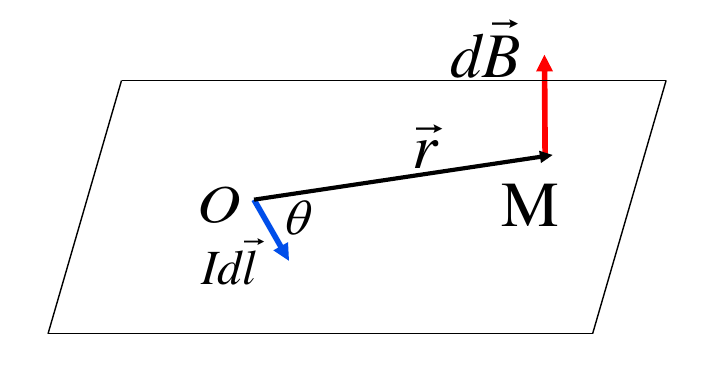
\includegraphics[width=0.4\textwidth]{ch04-1.png}
\end{figure*}

\subsubsection{Áp dụng cảm ứng từ dòng điện thẳng}

\begin{figure}[h]
  \centering
  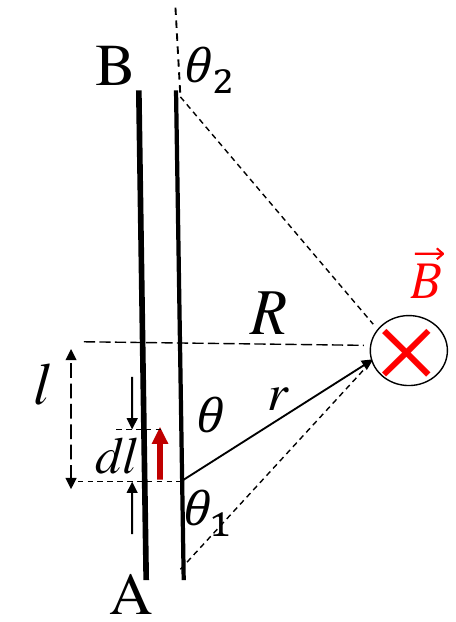
\includegraphics[width=0.4\textwidth]{ch04-2.png}
\end{figure}

\begin{gather*}
  dB = \frac{\mu_0\mu}{4\pi} \frac{Idl\sin\theta}{r^2} \\
  B = \int_{AB} dB = \dots = \frac{\mu_0\mu I}{4\pi R} \left( \cos \theta_1 - \cos \theta_2 \right)
\end{gather*}

Dòng vô tận có 
\begin{equation*}
  B = \frac{\mu_0\mu I}{2\pi R}
\end{equation*}

\subsection[Câu 3]{Câu 3: Xác định vector cảm ứng từ gây bởi dòng điện tròn có cường độ $I$, bán kính $R$, tại điểm $M$ nằm trên trục của dòng điện, cách tâm $O$ của dòng điện một
khoảng $h$. Từ kết quả trên xét hai trường hợp giới hạn:
\begin{itemize}
    \item M trùng với tâm O của dòng điện ($h = 0$)
    \item M ở rất xa dòng điện ($h \gg R$).
\end{itemize}
}

Tính cảm ứng từ gây bởi dòng điện tròn (tự làm):

\begin{equation*}
  \vec{B} = \frac{\mu_0 \mu I \vec{S}}{2\pi (R^2 + h^2)^{\frac{3}{2}}}
\end{equation*}

\begin{itemize}
  \item Ở tâm thì $B = \frac{\mu_0 \mu I}{2R}$
  \item Ở xa thì $B = \frac{\mu_0 \mu IS}{2\pi h^3}$
\end{itemize}

\subsection[Câu 4]{Câu 4: Phát biểu, viết biểu thức và nêu ý nghĩa của định lý Ampe về lưu số của vector cường độ từ trường. Áp dụng định lý Ampe để xác định biểu thức cảm ứng từ trong lòng cuộn dây điện hình xuyến và trong lòng ống dây điện thẳng dài vô hạn mang dòng điện $I$.}

Định lý Ampe về lưu số của vector cường độ từ trường: Lưu số của vector cường độ từ trường dọc theo một đường cong kín bằng tổng đại số cường độ các dòng điện xuyên qua phần diện tích giới hạn bởi đường cong đó.

\begin{equation*}
  \oint_C \vec{H}d\vec{l} = \sum I_i
\end{equation*}

Ý nghĩa: Cho ta biết rằng từ trường là một trường xoáy

\begin{itemize}
  \item Cảm ứng từ trong lòng cuộn dây hình xuyến $n$ vòng, bán kính $R$: $B = \frac{\mu_0 \mu nI}{2\pi R}$
  \item Cảm ứng từ trong lòng cuộn dây dài vô tận: $B = \mu_0\mu n_0I$
\end{itemize}

\subsection[Câu 5]{Câu 5: Trình bày:
\begin{enumerate}
    \item Khái niệm đường sức từ trường
    \item Định nghĩa từ thông qua diện tích $S$
    \item Phát biểu, viết biểu thức và nêu ý nghĩa của định lý O-G đối với từ trường
\end{enumerate}}

\subsubsection{Khái niệm đường sức từ trường}

Đường sức từ trường (hay đường cảm ứng từ) là đường cong trong từ trường mà tiếp tuyến tại mọi điểm trùng với phương của vector cảm ứng từ tại điểm đó, chiều của đường cảm ứng từ là chiều của vector cảm ứng từ

\subsubsection{Định nghĩa từ thông}

Từ thông qua diện tích $dS$ là đại lượng có trị số bằng 

\begin{equation*}
  d\Phi = \vec{B}d\vec{S}
\end{equation*}

Từ thông qua diện tích $dS$ vè trị số là số đường cảm ứng từ qua diện tích ấy.

Tìm từ thông qua diện tích $S$, ta chia thành các diện tích nhỏ $dS$ sao cho $\vec{B}$ trên mỗi diện tích ấy coi như không đổi.

\begin{equation*}
  \Phi = \int_S d\Phi = \int_S \vec{B}d\vec{S}
\end{equation*}

\subsubsection{Định lý O-G trong từ trường}

Từ thông toàn phần gửi qua mặt kín bất kỳ bằng 0

\begin{equation*}
  \oint_S \vec{B}d\vec{S} = 0
\end{equation*}

Ý nghĩa: Từ trường là một trường xoáy. Trong tự nhiên không tồn tại các hạt mang từ tính.

\subsection[Câu 6]{Câu 6: Trình bày tác dụng của từ trường đều lên một mạch điện kín (mạch kín là một khung dây dẫn cứng hình chữ nhật có dòng điện cường độ $I$ chạy qua) trong trường hợp cảm ứng từ hợp với véctơ pháp tuyến mặt phẳng khung một góc $\alpha$.}

\begin{figure}[h]
  \centering
  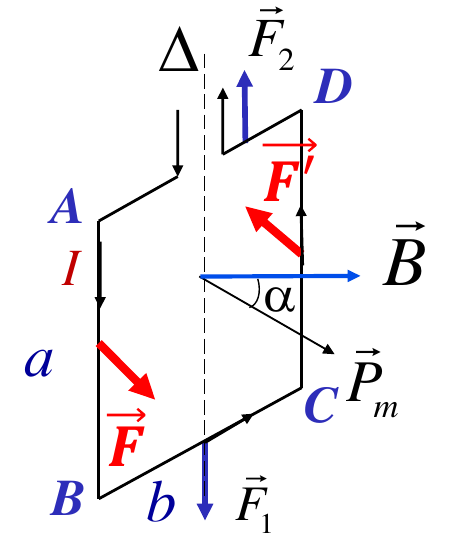
\includegraphics[width=0.4\textwidth]{ch04-3.png}
\end{figure}

Xét khung dây hình chữ nhật có 2 cạnh $a, b$ và dòng $I$

\begin{itemize}
  \item Khung đặt trong từ trường đều $\vec{B}$ có phương vuông góc với $AB, CD$
  \item Khung quay quanh trục $\Delta$
  \item Ban đầu mặt phẳng khung không vuông góc với từ trường
\end{itemize}

Từ lực lên khung có $\sum \vec{F} = \vec{F}_1 + \vec{F}_2 + \vec{F} + \vec{F}'$

\begin{itemize}
  \item $\vec{F}_1 + \vec{F}_2 = \vec{0}$. Phản lực triệt tiêu 
  \item $F = F' = IaB$, tạo thành ngẫu lực khiến khung quay quanh $\Delta$ cho đến khi mặt phẳng khung vuông góc với từ trường
  \item Khung quay theo chiều giảm $\alpha$
\end{itemize}

Khi đó momen ngẫu lực đối với trục $\Delta$ là 

\begin{equation*}
  \mu = Fd = IaB \cdot b\sin\alpha = ISB\sin\alpha = P_m B \sin\alpha
\end{equation*}

Chiều momen ngẫu lực vuông góc với mp chứa $\vec{P}_m$ và $\vec{B}$

\begin{equation*}
  \vec{\mu} = \vec{P}_m \times \vec{B}
\end{equation*}

Năng lượng khung dây trong từ trường:

\begin{equation*}
  W_m(\alpha) = -P_mB\cos\alpha = -\vec{P}_m\vec{B}
\end{equation*}

\subsection[Câu 7]{Câu 7: Trình bày về lực Lorentz tác dụng lên hạt mang điện chuyển động trong từ trường có cảm ứng từ $\vec{B}$. Thành lập phương trình chuyển động của hạt mang điện $q$, khối lượng $m$, chuyển động vận tốc $\vec{v}$ dưới tác dụng của từ trường $\vec{B}$ (góc giữa $\vec{v}$ và $\vec{B}$ là $\alpha$)}

Xét hạt điện $q$ chuyển động với vận tốc $\vec{v}$ trong từ trường $\vec{B}$

\begin{itemize}
  \item Hạt điện chuyển động tương đương phần từ điện tích $Id\vec{l} = q\vec{v}$
  \item Từ lực lên phần tử dòng điện: $d\vec{F} = Id\vec{l} \times \vec{B}$
  \item Lực Lorentz tác dụng lên hạt điện: $\vec{F}_L = q\vec{v} \times \vec{B}$
\end{itemize}

Lực Lorentz: 

\begin{itemize}
  \item Đặt tại hạt điện $q$
  \item Phương vuông góc với phương chuyển động của $q$ và $\vec{B}$
  \item Chiều sao cho $q\vec{v}, \vec{B}, \vec{F}_L$ tạo tam diện thuận
  \item Độ lớn $|F_L| = |q|vB\sin\alpha$
\end{itemize}

Trường hợp chuyển động với góc $\alpha$: Chia $\vec{v}$ thành 2 thành phần $\vec{v}_{//}$ và $\vec{v}_{\perp}$

Khi đó trong mp vuông góc với $\vec{B}$ thì $q$ chuyển động trên đường tròn:

\begin{equation*}
  R = \frac{mv_{\perp}}{|q|B} = \frac{mv\sin\alpha}{|q|B}
\end{equation*}

Quỹ đạo của hạt là hình xoắn ốc với bước

\begin{equation*}
  h = v_{//}T = \frac{2\pi mv\cos\alpha}{|q|B}
\end{equation*}